\section{Relationships of organisms with one another and with the environment}
\subsection{Energy flow}
Sun is the principal source of energy input to most biological systems. 

The energy from the sun
is captured into glucose by photosynthesis, that energy is then passed onto other organisms and so
every animal on earth is dependent on photosynthesis.

\begin{center}
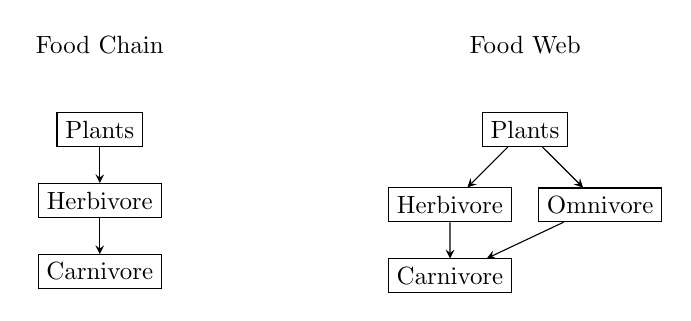
\begin{tikzpicture}[scale=1.2, every node/.style={scale=0.9}, ->,>=stealth]

% Food Chain
\node[rectangle, draw, align=center] (plant) {Plants};
\node[rectangle, draw, below of=plant, node distance=1cm, align=center] (herbivore) {Herbivore};
\node[rectangle, draw, below of=herbivore, node distance=1cm, align=center] (carnivore1) {Carnivore};

\draw[->] (plant) -- (herbivore);
\draw[->] (herbivore) -- (carnivore1);

% Label for Food Chain
\node[above of=plant, node distance=1.2cm] {Food Chain};

% Food Web
\node[rectangle, draw, right of=plant, node distance=6cm, align=center] (plant2) {Plants};
\node[rectangle, draw, below left of=plant2, node distance=1.5cm, align=center] (herbivore2) {Herbivore};
\node[rectangle, draw, below right of=plant2, node distance=1.5cm, align=center] (omnivore) {Omnivore};
\node[rectangle, draw, below of=herbivore2, node distance=1cm, align=center] (carnivore2) {Carnivore};

\draw[->] (plant2) -- (herbivore2);
\draw[->] (plant2) -- (omnivore);
\draw[->] (herbivore2) -- (carnivore2);
\draw[->] (omnivore) -- (carnivore2);

% Label for Food Web
\node[above of=plant2, node distance=1.2cm] {Food Web};

\end{tikzpicture}
\end{center}
Using the two diagramatic structures above, energy flow from one organism to another can be 
represented. A food chain is a diagram showing the flow of energy from one organism to another.
 food web shows that but in multiple interconnected food chains. Both diagrams begin at producers.
Each stage in a food wave or food chain is called a trophic level.

Producers are organisms that make their own organic nutrients, generally using energy from 
sunlight, through photosynthesis. Consumers are organisms that eat these producers to get their
nutrients. 

Herbivores are animals that feed on plants, carnivores are animals that feed on animals.

A decomposer is an organism that gets its energy from dead or waste organic material.

The transfer of energy from one trophic level to another is inefficient for the following reasons:
\begin{itemize}
	\item The organism being eaten has itself respired some of the energy.
	\item Not all of the organism is eaten
	\item Not all of the eaten part of the organism is digested
\end{itemize}

Those that eat consumers are called primary consumers, they are also herbivores. Those that eat
primary consumers are secondary and so on tertiary and quaternary. There are rarely more than five
trophic levels.

In terms of just energy, it is more efficient for humans to eat crops than to eat animals raised on
crops, as energy is lost in two stages when we eat animals, that during photosynthesis from the sun
and that during eating by the animals. Crops provide energy directly captured from the sun and 
hence eating crops is more efficient.

\begin{center}
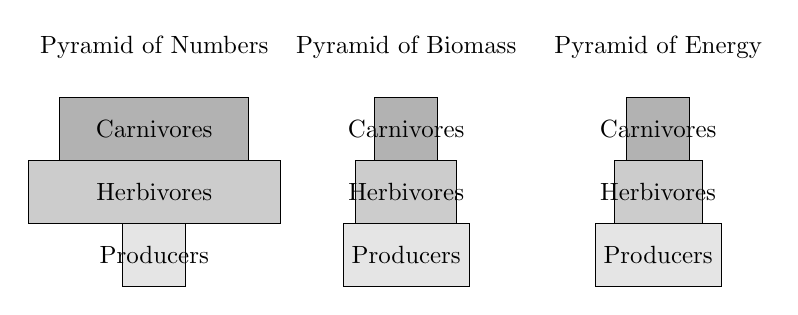
\begin{tikzpicture}[scale=0.8, every node/.style={scale=0.9}, ->,>=stealth]

% Label for Pyramid of Numbers
\node at (0,3.8) {Pyramid of Numbers};

% Pyramid of Numbers (Producers smallest)
\draw[fill=black!10] (-0.5,0) rectangle (0.5,1);  % Producers (smallest)
\draw[fill=black!20] (-2,1) rectangle (2,2);  % Herbivores
\draw[fill=black!30] (-1.5,2) rectangle (1.5,3);  % Carnivores

% Labels inside the boxes for Pyramid of Numbers
\node at (0,0.5) {Producers};
\node at (0,1.5) {Herbivores};
\node at (0,2.5) {Carnivores};

% Label for Pyramid of Biomass
\node at (4,3.8) {Pyramid of Biomass};

% Pyramid of Biomass (Even levels)
\draw[fill=black!10] (3,0) rectangle (5,1);  % Producers
\draw[fill=black!20] (3.2,1) rectangle (4.8,2);  % Herbivores
\draw[fill=black!30] (3.5,2) rectangle (4.5,3);  % Carnivores

% Labels inside the boxes for Pyramid of Biomass
\node at (4,0.5) {Producers};
\node at (4,1.5) {Herbivores};
\node at (4,2.5) {Carnivores};

% Label for Pyramid of Energy
\node at (8,3.8) {Pyramid of Energy};

% Pyramid of Energy (Even levels)
\draw[fill=black!10] (7,0) rectangle (9,1);  % Producers
\draw[fill=black!20] (7.3,1) rectangle (8.7,2);  % Herbivores
\draw[fill=black!30] (7.5,2) rectangle (8.5,3);  % Carnivores

% Labels inside the boxes for Pyramid of Energy
\node at (8,0.5) {Producers};
\node at (8,1.5) {Herbivores};
\node at (8,2.5) {Carnivores};

\end{tikzpicture}
\end{center}
Above are diagrams for the pyramids of numbers, biomass and energy. The pyramid of numbers is
uneven because there may be one huge producer, such as a tree upon which many herbivores depend.

The pyramids of biomass represent the mass of each trophic level and are hence evenly shaped 
because no matter the number of the organisms, the mass will be directly proportional to the
energy at that trophic level.

The pyramid of energy represents the energy at each trophic level.
